\documentclass[11pt,ignorenonframetext,]{beamer}
\setbeamertemplate{caption}[numbered]
\setbeamertemplate{caption label separator}{: }
\setbeamercolor{caption name}{fg=normal text.fg}
\beamertemplatenavigationsymbolsempty
\usepackage{lmodern}
\usepackage{amssymb,amsmath}
\usepackage{ifxetex,ifluatex}
\usepackage{fixltx2e} % provides \textsubscript
\ifnum 0\ifxetex 1\fi\ifluatex 1\fi=0 % if pdftex
  \usepackage[T1]{fontenc}
  \usepackage[utf8]{inputenc}
\else % if luatex or xelatex
  \ifxetex
    \usepackage{mathspec}
  \else
    \usepackage{fontspec}
  \fi
  \defaultfontfeatures{Ligatures=TeX,Scale=MatchLowercase}
\fi
\usetheme[]{metropolis}
% use upquote if available, for straight quotes in verbatim environments
\IfFileExists{upquote.sty}{\usepackage{upquote}}{}
% use microtype if available
\IfFileExists{microtype.sty}{%
\usepackage{microtype}
\UseMicrotypeSet[protrusion]{basicmath} % disable protrusion for tt fonts
}{}
\newif\ifbibliography
\hypersetup{
            pdftitle={Lecture 7},
            pdfauthor={Colin Rundel},
            pdfborder={0 0 0},
            breaklinks=true}
\urlstyle{same}  % don't use monospace font for urls
\usepackage{graphicx,grffile}
\makeatletter
\def\maxwidth{\ifdim\Gin@nat@width>\linewidth\linewidth\else\Gin@nat@width\fi}
\def\maxheight{\ifdim\Gin@nat@height>\textheight0.8\textheight\else\Gin@nat@height\fi}
\makeatother
% Scale images if necessary, so that they will not overflow the page
% margins by default, and it is still possible to overwrite the defaults
% using explicit options in \includegraphics[width, height, ...]{}
\setkeys{Gin}{width=\maxwidth,height=\maxheight,keepaspectratio}

% Prevent slide breaks in the middle of a paragraph:
\widowpenalties 1 10000
\raggedbottom

\AtBeginPart{
  \let\insertpartnumber\relax
  \let\partname\relax
  \frame{\partpage}
}
\AtBeginSection{
  \ifbibliography
  \else
    \let\insertsectionnumber\relax
    \let\sectionname\relax
    \frame{\sectionpage}
  \fi
}
\AtBeginSubsection{
  \let\insertsubsectionnumber\relax
  \let\subsectionname\relax
  \frame{\subsectionpage}
}

\setlength{\parindent}{0pt}
\setlength{\parskip}{6pt plus 2pt minus 1pt}
\setlength{\emergencystretch}{3em}  % prevent overfull lines
\providecommand{\tightlist}{%
  \setlength{\itemsep}{0pt}\setlength{\parskip}{0pt}}
\setcounter{secnumdepth}{0}

\usepackage{geometry}
\usepackage{graphicx}
\usepackage{amssymb}
\usepackage{color}          	% gives color options
\usepackage{url}		% produces hyperlinks
\usepackage[english]{babel}
\usepackage{colortbl}	% allows for color usage in tables
\usepackage{multirow}	% allows for rows that span multiple rows in tables
\usepackage{xcolor}		% this package has a variety of color options
\usepackage{calc}
\usepackage{multicol}
\usepackage{wrapfig}
\usepackage{textcomp}
\usepackage{bm}
\usepackage{bbm}
\usepackage{setspace}
\singlespacing

%%%%%%%%%%%%%%%%
% Small code output
%%%%%%%%%%%%%%%%

%% change fontsize of R code

%\let\oldShaded\Shaded
%\let\endoldShaded\endShaded
%\renewenvironment{Shaded}{\footnotesize\begin{spacing}{0.9}\oldShaded}{\endoldShaded\end{spacing}}

%% change fontsize of output
\let\oldverbatim\verbatim
\let\endoldverbatim\endverbatim
\renewenvironment{verbatim}{\footnotesize\begin{spacing}{0.9}\oldverbatim}{\endoldverbatim\end{spacing}}


\newcommand{\verbatimfont}[1]{\renewcommand{\verbatim@font}{\ttfamily#1}}

%%%%%%%%%%%%%%%%
% Custom Colors
%%%%%%%%%%%%%%%%

\xdefinecolor{oiBlue}{rgb}{0.15, 0.35, 0.55}
\xdefinecolor{gray}{rgb}{0.5, 0.5, 0.5}
\xdefinecolor{darkGray}{rgb}{0.3, 0.3, 0.3}
\xdefinecolor{darkerGray}{rgb}{0.2, 0.2, 0.2}
\xdefinecolor{rubineRed}{rgb}{0.89,0,0.30}
\xdefinecolor{linkCol}{rgb}{0.11,0.49,0.95}	
\xdefinecolor{irishGreen}{rgb}{0,0.60,0}	
\xdefinecolor{darkturquoise}{rgb}{0.44, 0.58, 0.86}
\definecolor{lightGreen}{rgb}{0.533,0.765,0.42}
%\xdefinecolor{hlblue}{rgb}{0.051,0.65,1}
\xdefinecolor{hlblue}{rgb}{ 0.055, 0.639, 0.831}
\definecolor{light}{rgb}{.337,.608,.741}
\definecolor{dark}{rgb}{.337,.608,.741}

\definecolor{cpink}{rgb}{0.93, 0.23, 0.51}

%%%%%%%%%%%%%%%%
% Custom Commands
%%%%%%%%%%%%%%%%

% text colors
\newcommand{\red}[1]{\textit{\textcolor{rubineRed}{#1}}}
\newcommand{\orange}[1]{\textit{\textcolor{orange}{#1}}}
\newcommand{\pink}[1]{\textit{\textcolor{rubineRed!90!white!50}{#1}}}
\newcommand{\green}[1]{\textit{\textcolor{irishGreen}{#1}}}
\newcommand{\blue}[1]{\textit{\textcolor{darkturquoise}{#1}}}
\newcommand{\light}[1]{\textcolor{light}{\textbf{#1}}}
\newcommand{\dark}[1]{\textcolor{dark}{#1}}
\newcommand{\gray}[1]{\textcolor{gray}{#1}}


% links: webURL, webLin, appLink
\newcommand{\webURL}[1]{\urlstyle{same}{\textit{\textcolor{linkCol}{\url{#1}}} }}
\newcommand{\webLink}[2]{\href{#1}{\textcolor{linkCol}{{#2}}}}
\newcommand{\appLink}[2]{\href{#1}{\textcolor{lightGreen!80!black!90}{{#2}}}}

% mail
\newcommand{\mail}[1]{\href{mailto:#1}{\textit{\textcolor{linkCol}{#1}}}}

% highlighting: hl, hlGr, mathhl
\newcommand{\hl}[1]{\textit{\textcolor{hlblue}{#1}}}
\newcommand{\hlGr}[1]{\textit{\textcolor{lightGreen}{#1}}}
\newcommand{\hlRd}[1]{\textit{\textcolor{rubineRed}{#1}}}
\newcommand{\mathhl}[1]{\textcolor{hlblue}{\ensuremath{#1}}}

% example
\newcommand{\ex}[1]{\textcolor{blue}{{{\small (#1)}}}}


\DeclareMathOperator*{\argmin}{arg\,min}
\DeclareMathOperator*{\argmax}{arg\,max}

\title{Lecture 7}
\subtitle{AR Models}
\author{Colin Rundel}
\date{02/08/2017}

\begin{document}
\frame{\titlepage}

\section{Lagged Predictors and CCFs}\label{lagged-predictors-and-ccfs}

\begin{frame}[fragile]{Southern Oscillation Index \& Recruitment}

The Southern Oscillation Index (SOI) is an indicator of the development
and intensity of El Niño (negative SOI) or La Niña (positive SOI) events
in the Pacific Ocean. These data also included the estimate of
``recruitment'', which indicate fish population sizes in the southern
hemisphere.

\begin{verbatim}
## # A tibble: 453 × 3
##        date    soi recruitment
##       <dbl>  <dbl>       <dbl>
## 1  1950.000  0.377       68.63
## 2  1950.083  0.246       68.63
## 3  1950.167  0.311       68.63
## 4  1950.250  0.104       68.63
## 5  1950.333 -0.016       68.63
## 6  1950.417  0.235       68.63
## 7  1950.500  0.137       59.16
## 8  1950.583  0.191       48.70
## 9  1950.667 -0.016       47.54
## 10 1950.750  0.290       50.91
## # ... with 443 more rows
\end{verbatim}

\end{frame}

\begin{frame}{Time series}

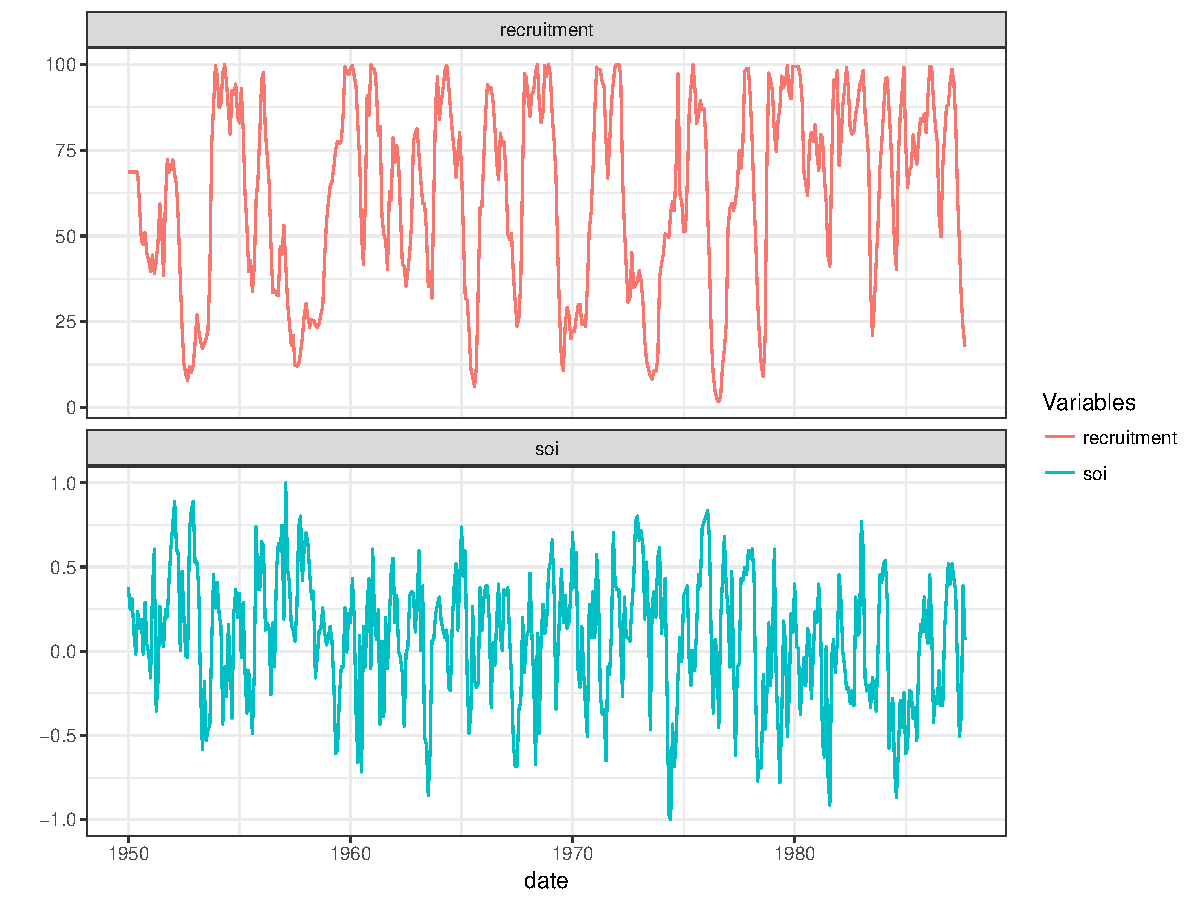
\includegraphics{Lec7_files/figure-beamer/unnamed-chunk-2-1.pdf}

\end{frame}

\begin{frame}{Relationship?}

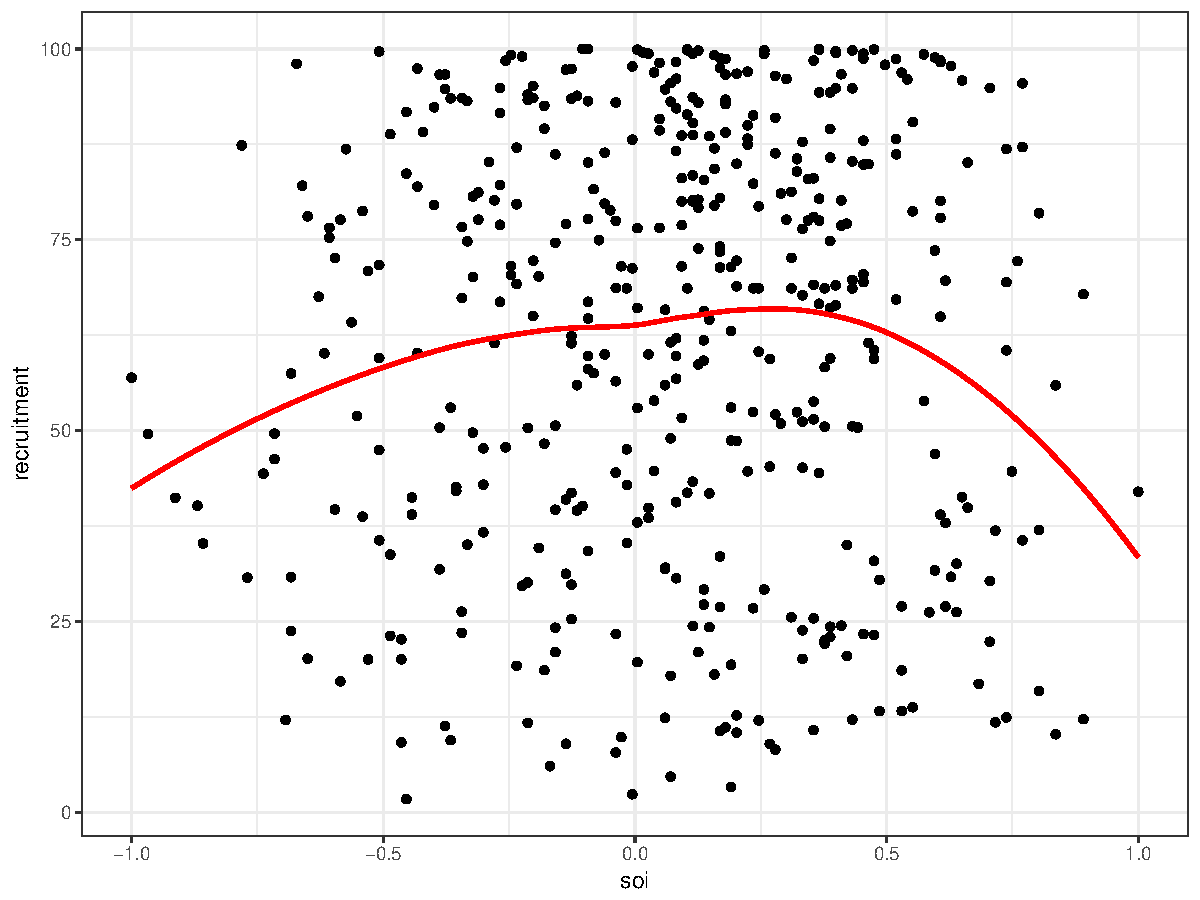
\includegraphics{Lec7_files/figure-beamer/unnamed-chunk-3-1.pdf}

\end{frame}

\begin{frame}{ACFs \& PACFs}

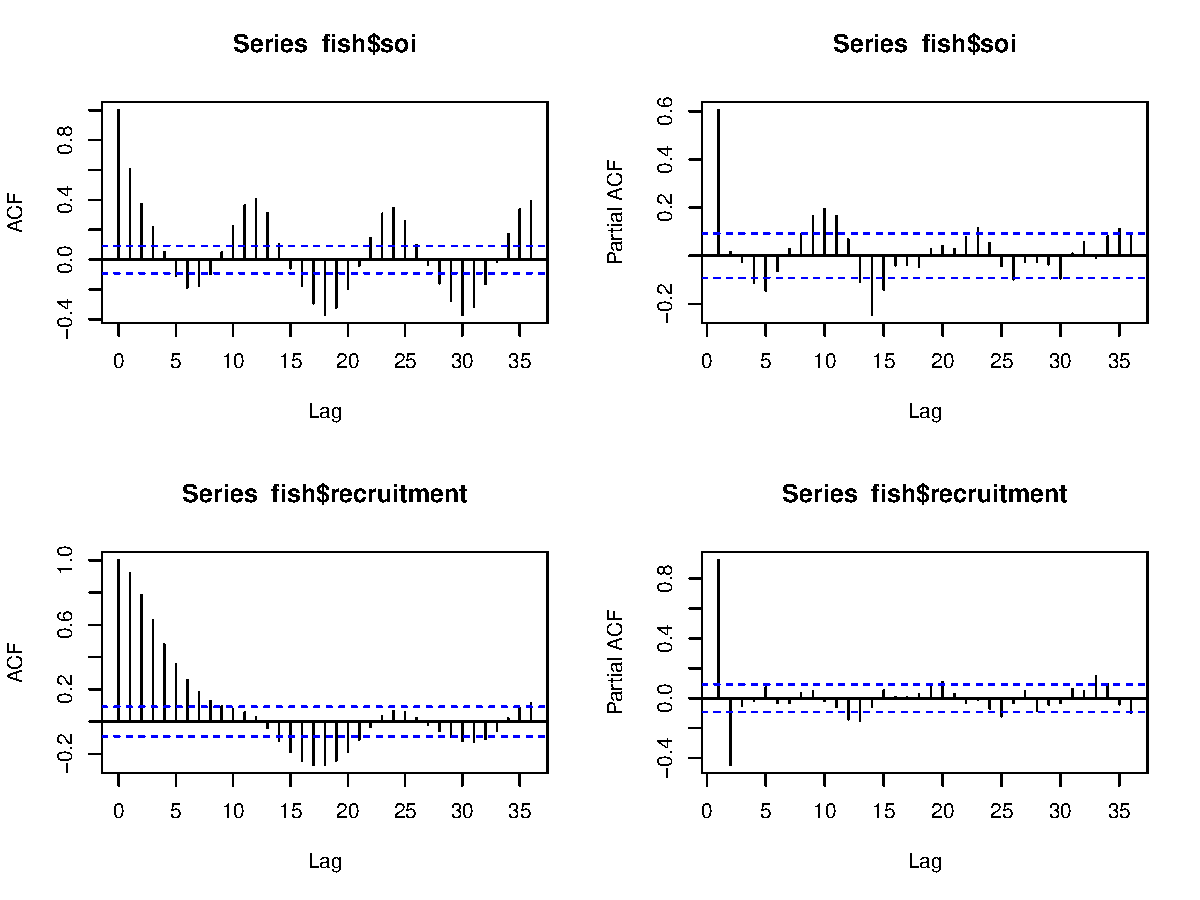
\includegraphics{Lec7_files/figure-beamer/unnamed-chunk-4-1.pdf}

\end{frame}

\begin{frame}{Cross correlation function}

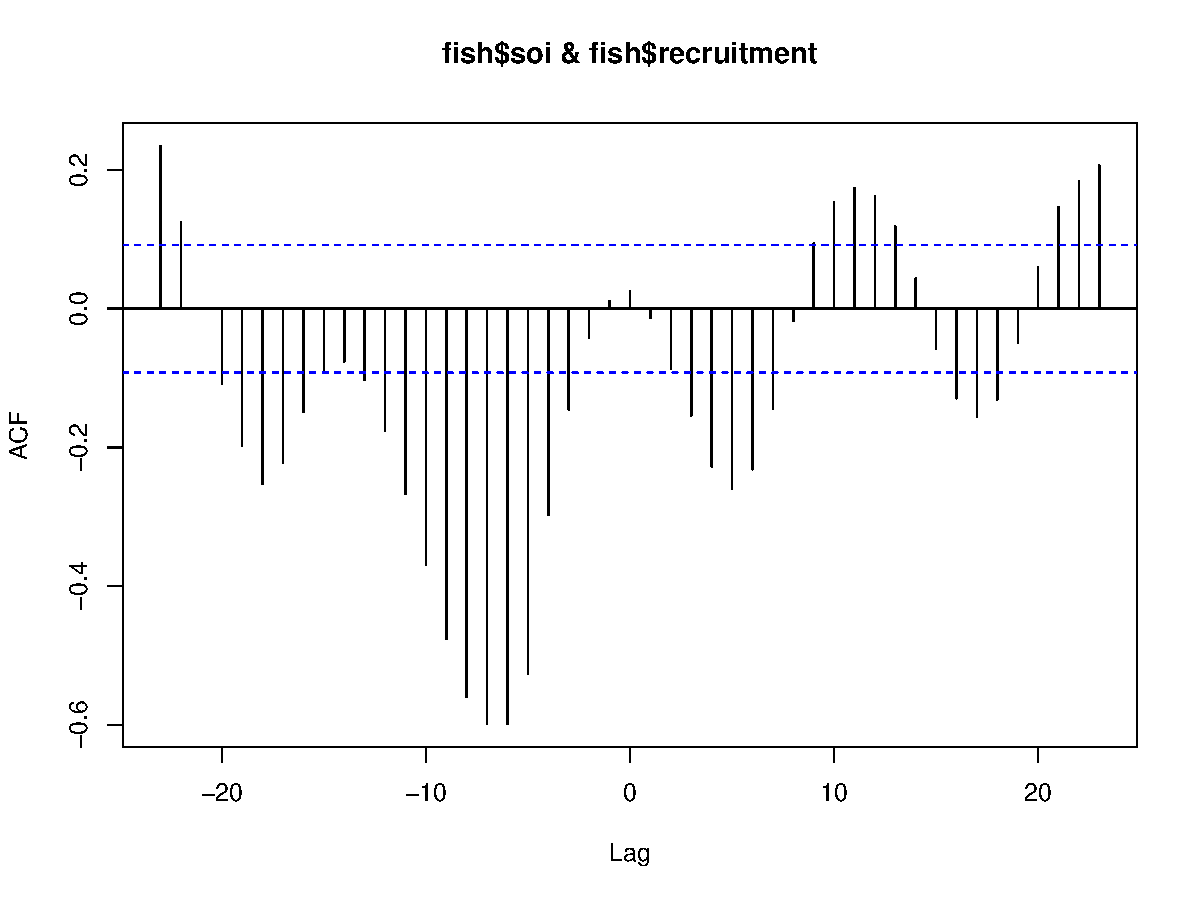
\includegraphics{Lec7_files/figure-beamer/unnamed-chunk-5-1.pdf}

\end{frame}

\begin{frame}{Cross correlation function - Scatter plots}

\begin{center}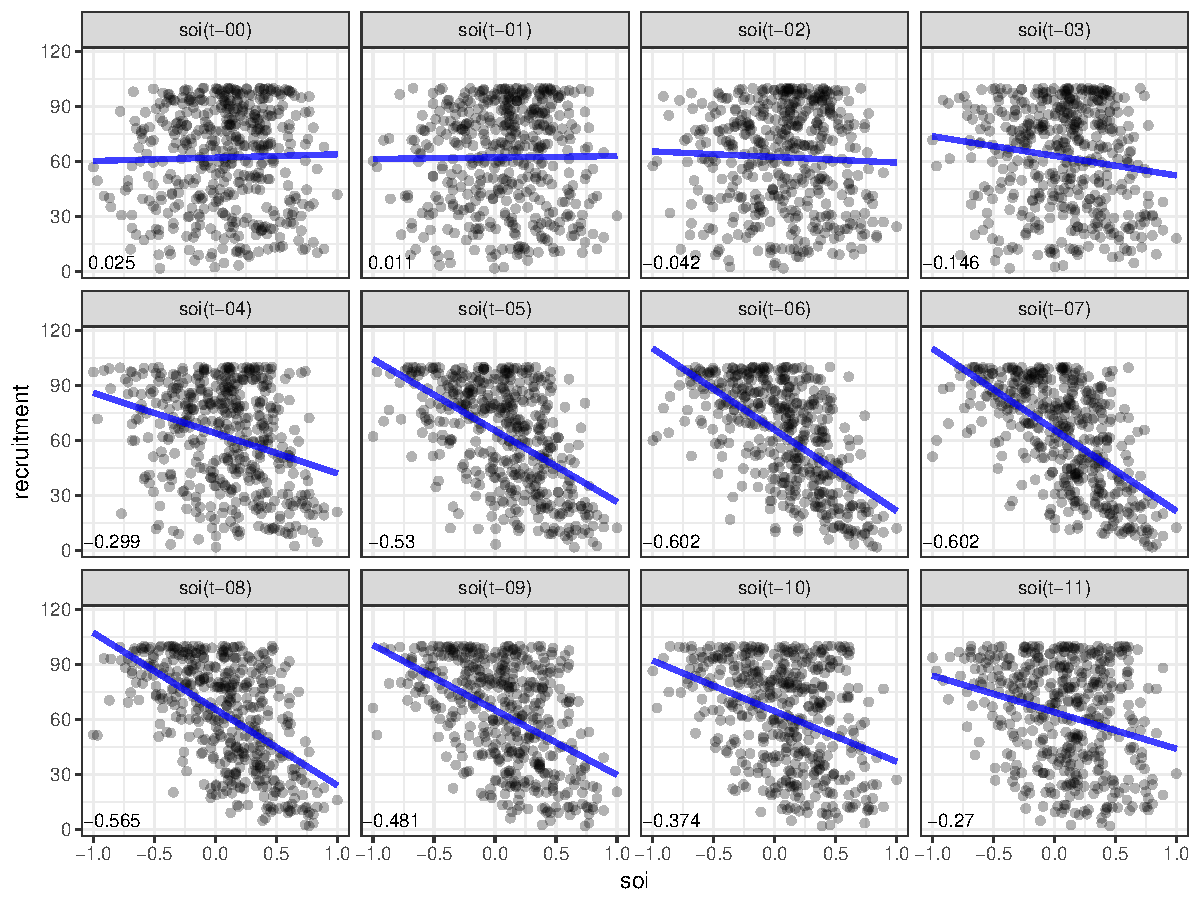
\includegraphics{Lec7_files/figure-beamer/unnamed-chunk-6-1} \end{center}

\end{frame}

\begin{frame}[fragile]{Model}

\begin{verbatim}
## 
## Call:
## lm(formula = recruitment ~ lag(soi, 5) + lag(soi, 6) + lag(soi, 
##     7) + lag(soi, 8), data = fish)
## 
## Residuals:
##     Min      1Q  Median      3Q     Max 
## -72.409 -13.527   0.191  12.851  46.040 
## 
## Coefficients:
##             Estimate Std. Error t value Pr(>|t|)    
## (Intercept)  67.9438     0.9306  73.007  < 2e-16 ***
## lag(soi, 5) -19.1502     2.9508  -6.490 2.32e-10 ***
## lag(soi, 6) -15.6894     3.4334  -4.570 6.36e-06 ***
## lag(soi, 7) -13.4041     3.4332  -3.904 0.000109 ***
## lag(soi, 8) -23.1480     2.9530  -7.839 3.46e-14 ***
## ---
## Signif. codes:  0 '***' 0.001 '**' 0.01 '*' 0.05 '.' 0.1 ' ' 1
## 
## Residual standard error: 18.93 on 440 degrees of freedom
##   (8 observations deleted due to missingness)
## Multiple R-squared:  0.5539, Adjusted R-squared:  0.5498 
## F-statistic: 136.6 on 4 and 440 DF,  p-value: < 2.2e-16
\end{verbatim}

\end{frame}

\begin{frame}{Prediction}

\begin{center}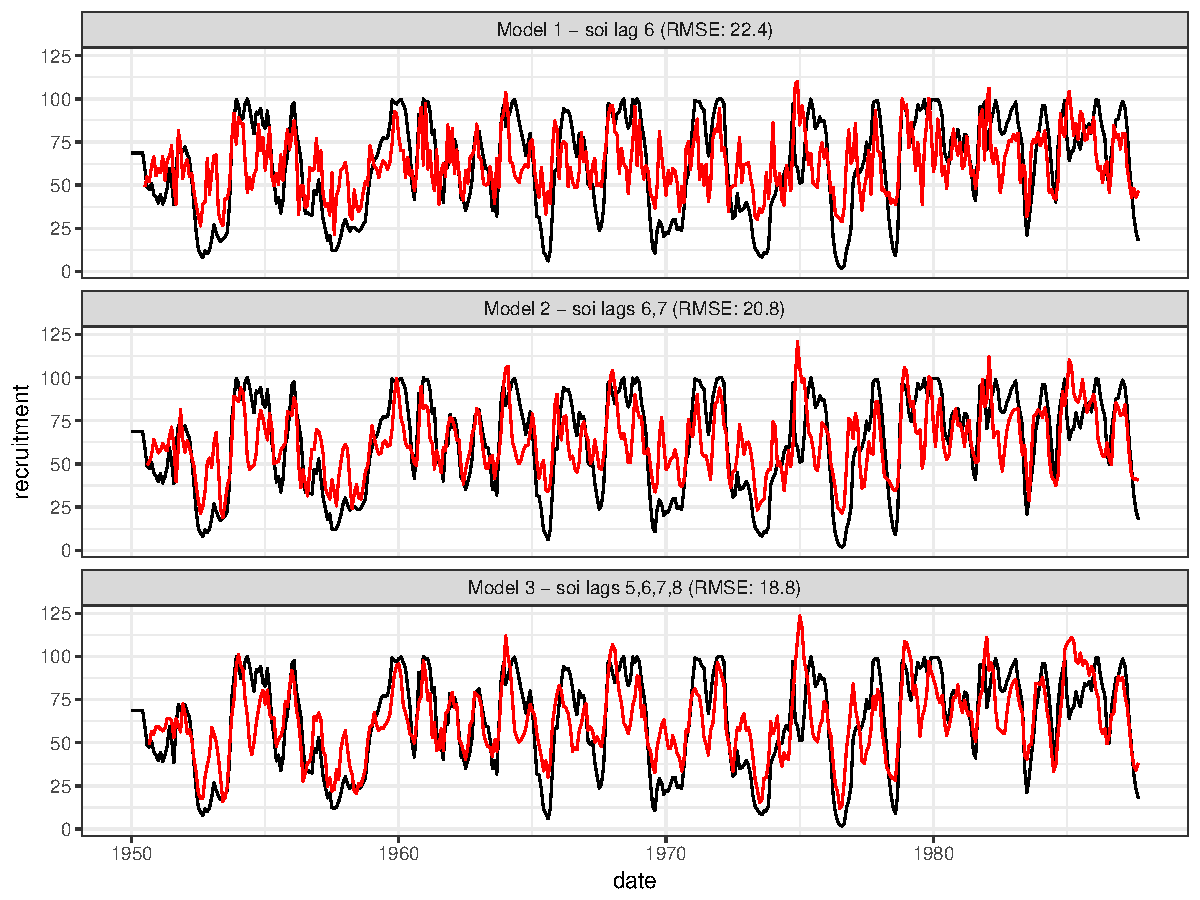
\includegraphics{Lec7_files/figure-beamer/unnamed-chunk-8-1} \end{center}

\end{frame}

\begin{frame}{Residual ACF - Model 3}

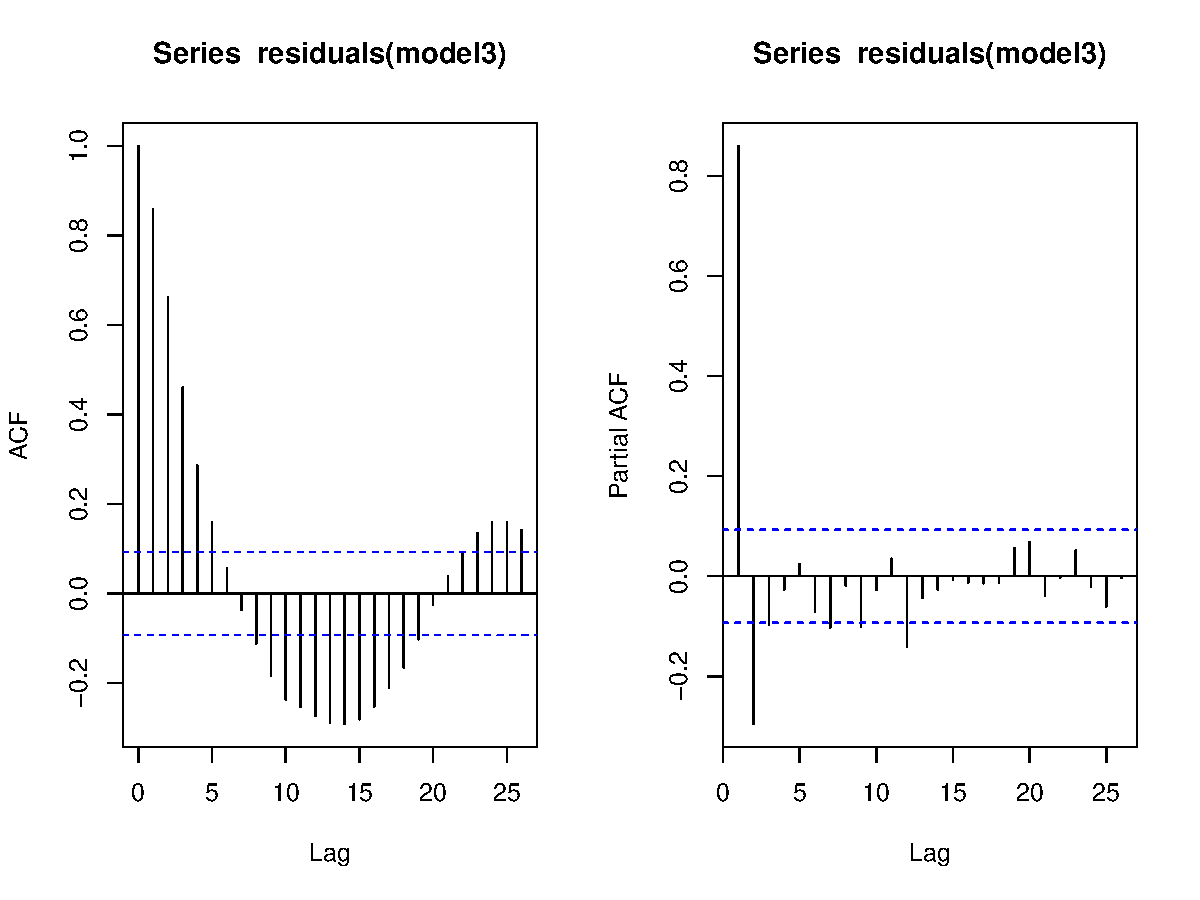
\includegraphics{Lec7_files/figure-beamer/unnamed-chunk-9-1.pdf}

\end{frame}

\begin{frame}[fragile]{Autoregessive model 1}

\begin{verbatim}
## 
## Call:
## lm(formula = recruitment ~ lag(recruitment, 1) + lag(recruitment, 
##     2) + lag(soi, 5) + lag(soi, 6) + lag(soi, 7) + lag(soi, 8), 
##     data = fish)
## 
## Residuals:
##     Min      1Q  Median      3Q     Max 
## -51.996  -2.892   0.103   3.117  28.579 
## 
## Coefficients:
##                      Estimate Std. Error t value Pr(>|t|)    
## (Intercept)          10.25007    1.17081   8.755  < 2e-16 ***
## lag(recruitment, 1)   1.25301    0.04312  29.061  < 2e-16 ***
## lag(recruitment, 2)  -0.39961    0.03998  -9.995  < 2e-16 ***
## lag(soi, 5)         -20.76309    1.09906 -18.892  < 2e-16 ***
## lag(soi, 6)           9.71918    1.56265   6.220 1.16e-09 ***
## lag(soi, 7)          -1.01131    1.31912  -0.767   0.4437    
## lag(soi, 8)          -2.29814    1.20730  -1.904   0.0576 .  
## ---
## Signif. codes:  0 '***' 0.001 '**' 0.01 '*' 0.05 '.' 0.1 ' ' 1
## 
## Residual standard error: 7.042 on 438 degrees of freedom
##   (8 observations deleted due to missingness)
## Multiple R-squared:  0.9385, Adjusted R-squared:  0.9377 
## F-statistic:  1115 on 6 and 438 DF,  p-value: < 2.2e-16
\end{verbatim}

\end{frame}

\begin{frame}[fragile]{Autoregessive model 2}

\begin{verbatim}
## 
## Call:
## lm(formula = recruitment ~ lag(recruitment, 1) + lag(recruitment, 
##     2) + lag(soi, 5) + lag(soi, 6), data = fish)
## 
## Residuals:
##     Min      1Q  Median      3Q     Max 
## -53.786  -2.999  -0.035   3.031  27.669 
## 
## Coefficients:
##                      Estimate Std. Error t value Pr(>|t|)    
## (Intercept)           8.78498    1.00171   8.770  < 2e-16 ***
## lag(recruitment, 1)   1.24575    0.04314  28.879  < 2e-16 ***
## lag(recruitment, 2)  -0.37193    0.03846  -9.670  < 2e-16 ***
## lag(soi, 5)         -20.83776    1.10208 -18.908  < 2e-16 ***
## lag(soi, 6)           8.55600    1.43146   5.977 4.68e-09 ***
## ---
## Signif. codes:  0 '***' 0.001 '**' 0.01 '*' 0.05 '.' 0.1 ' ' 1
## 
## Residual standard error: 7.069 on 442 degrees of freedom
##   (6 observations deleted due to missingness)
## Multiple R-squared:  0.9375, Adjusted R-squared:  0.937 
## F-statistic:  1658 on 4 and 442 DF,  p-value: < 2.2e-16
\end{verbatim}

\end{frame}

\begin{frame}{Prediction}

\begin{center}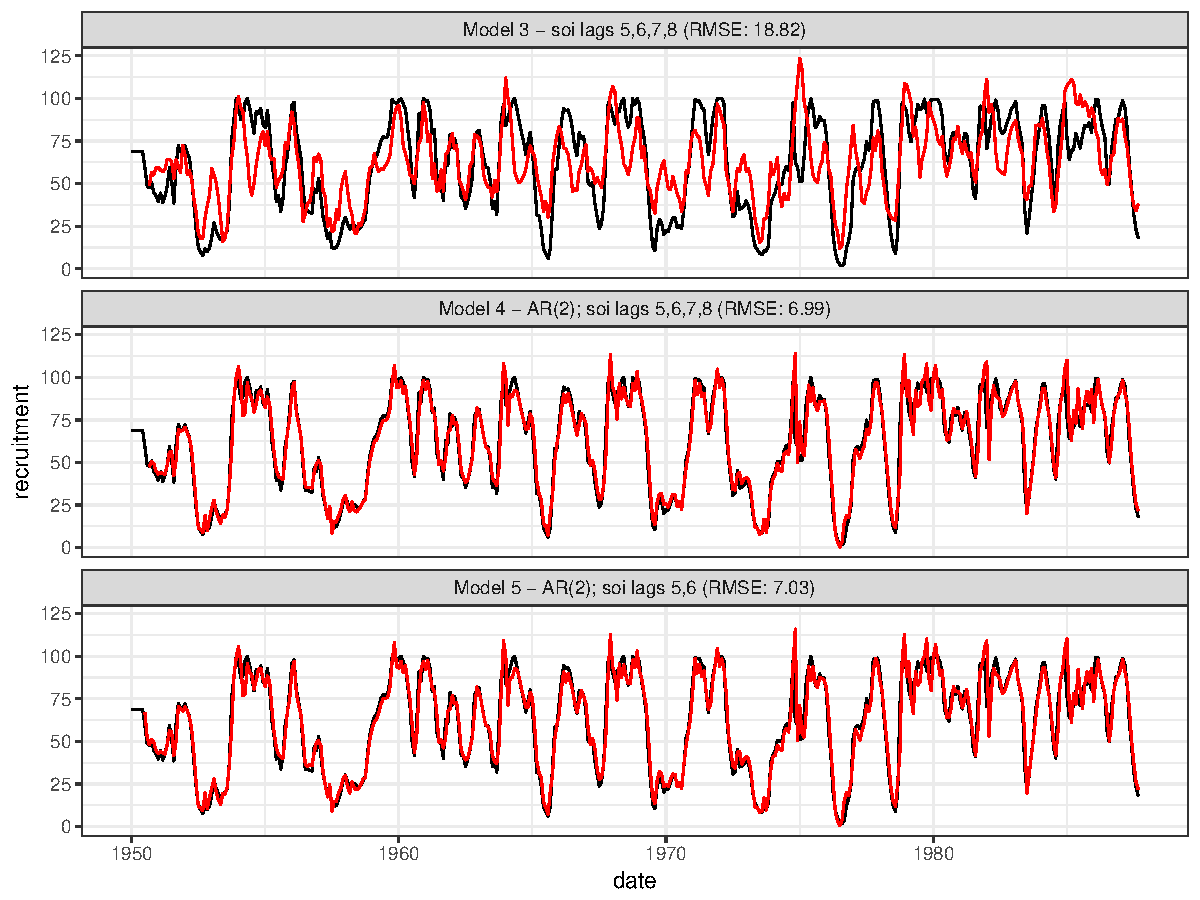
\includegraphics{Lec7_files/figure-beamer/unnamed-chunk-12-1} \end{center}

\end{frame}

\begin{frame}{Residual ACF - Model 5}

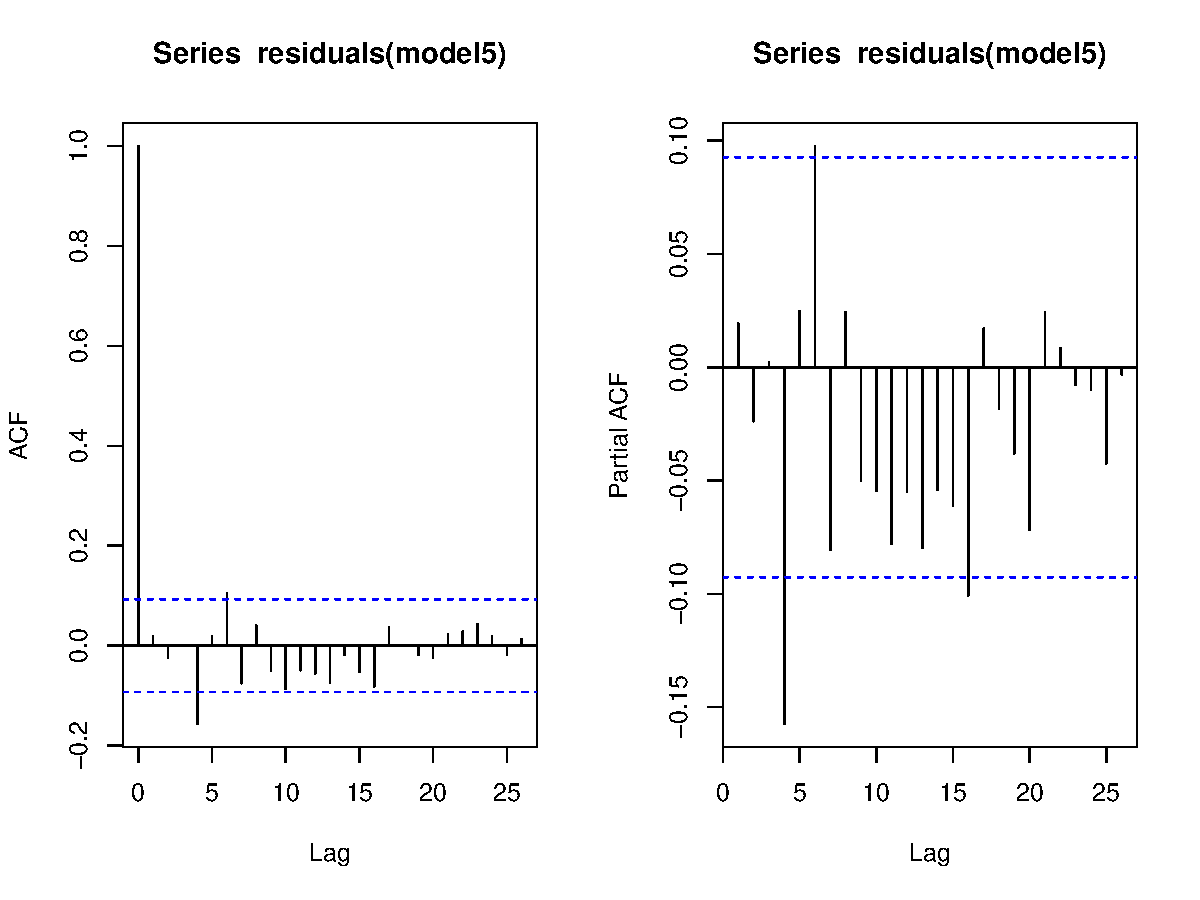
\includegraphics{Lec7_files/figure-beamer/unnamed-chunk-13-1.pdf}

\end{frame}

\section{Non-stationarity}\label{non-stationarity}

\begin{frame}[t]{Non-stationary models}

\vspace{5mm}

\begin{quote}
All happy families are alike; each unhappy family is unhappy in its own
way. - Tolstoy, Anna Karenina
\end{quote}

This applies to time series models as well, just replace happy family
with stationary model.

\pause

\vspace{3mm}

A simple example of a non-stationary time series is a trend stationary
model

\[ y_t = \mu_t + w_t \]

where \(\mu_t\) denotes the trend and \(w_t\) is a stationary process.

\pause

We've already been using this approach, since it is the same as
estimating \(\mu_t\) via regression and then examining the residuals
(\(\hat{w}_t = y_t - \hat{mu}_t\)) for stationarity.

\end{frame}

\begin{frame}{Linear trend model}

Lets imagine a simple model where \(y_t = \delta + \phi t + w_t\) where
\(\delta\) and \(\phi\) are constants and
\(w_t \sim \mathcal{N}(0,\sigma^2_w)\).

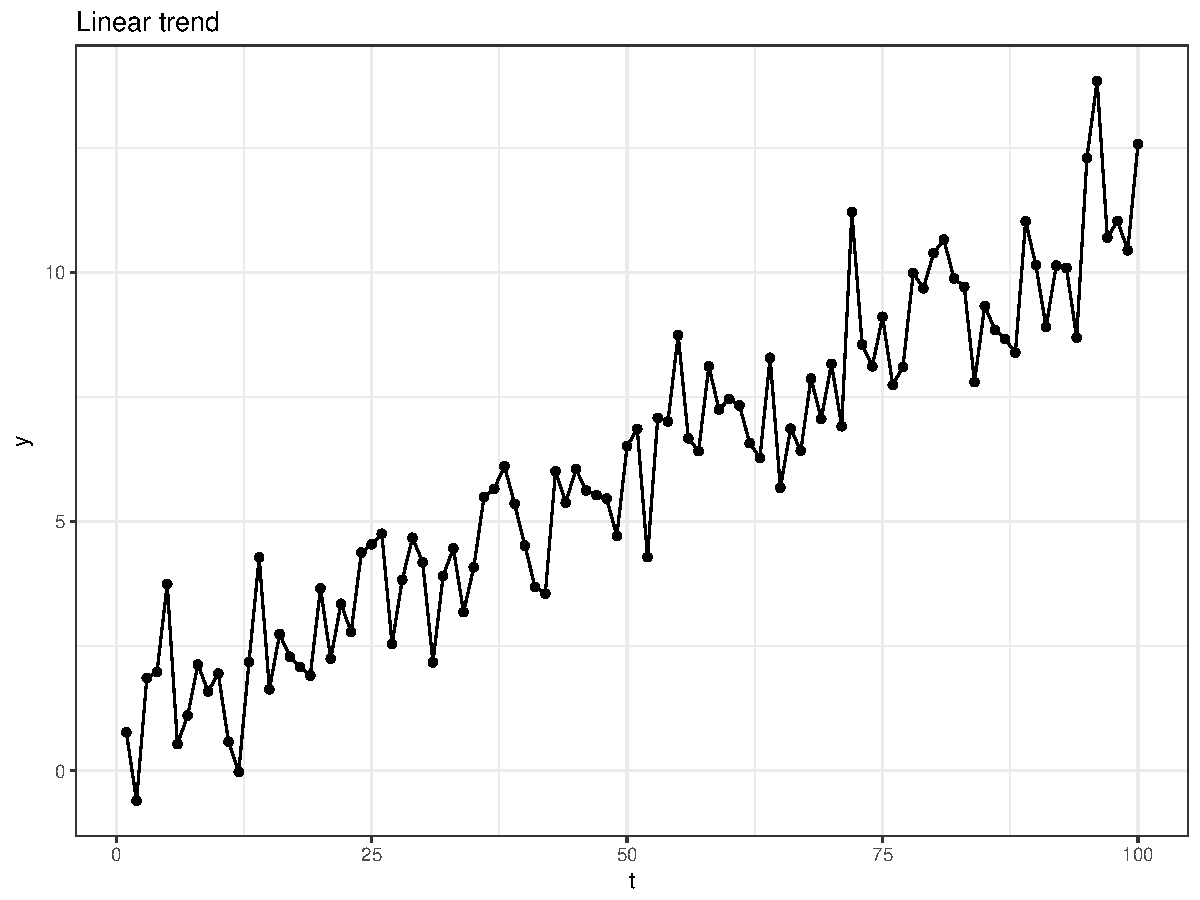
\includegraphics{Lec7_files/figure-beamer/unnamed-chunk-14-1.pdf}

\end{frame}

\begin{frame}[t]{Differencing}

An alternative approach to what we have seen is to examine the
differences of your response variable, specifically \(y_t - y_{t-1}\).

\end{frame}

\begin{frame}{Detrending vs Difference}

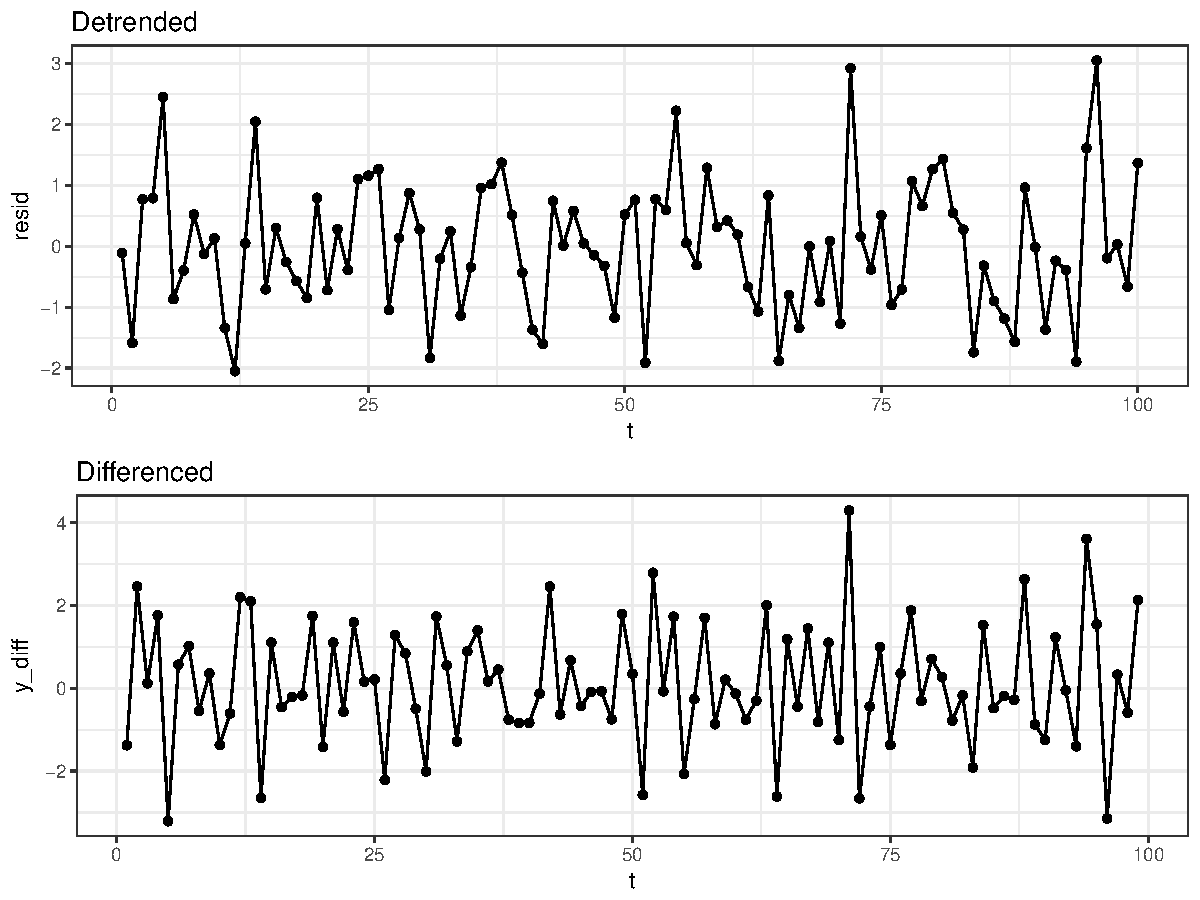
\includegraphics{Lec7_files/figure-beamer/unnamed-chunk-15-1.pdf}

\end{frame}

\begin{frame}{Quadratic trend model}

Lets imagine another simple model where
\(y_t = \delta + \phi t + \gamma t^2 + w_t\) where \(\delta\), \(\phi\),
and \(\gamma\) are constants and \(w_t \sim \mathcal{N}(0,\sigma^2_w)\).

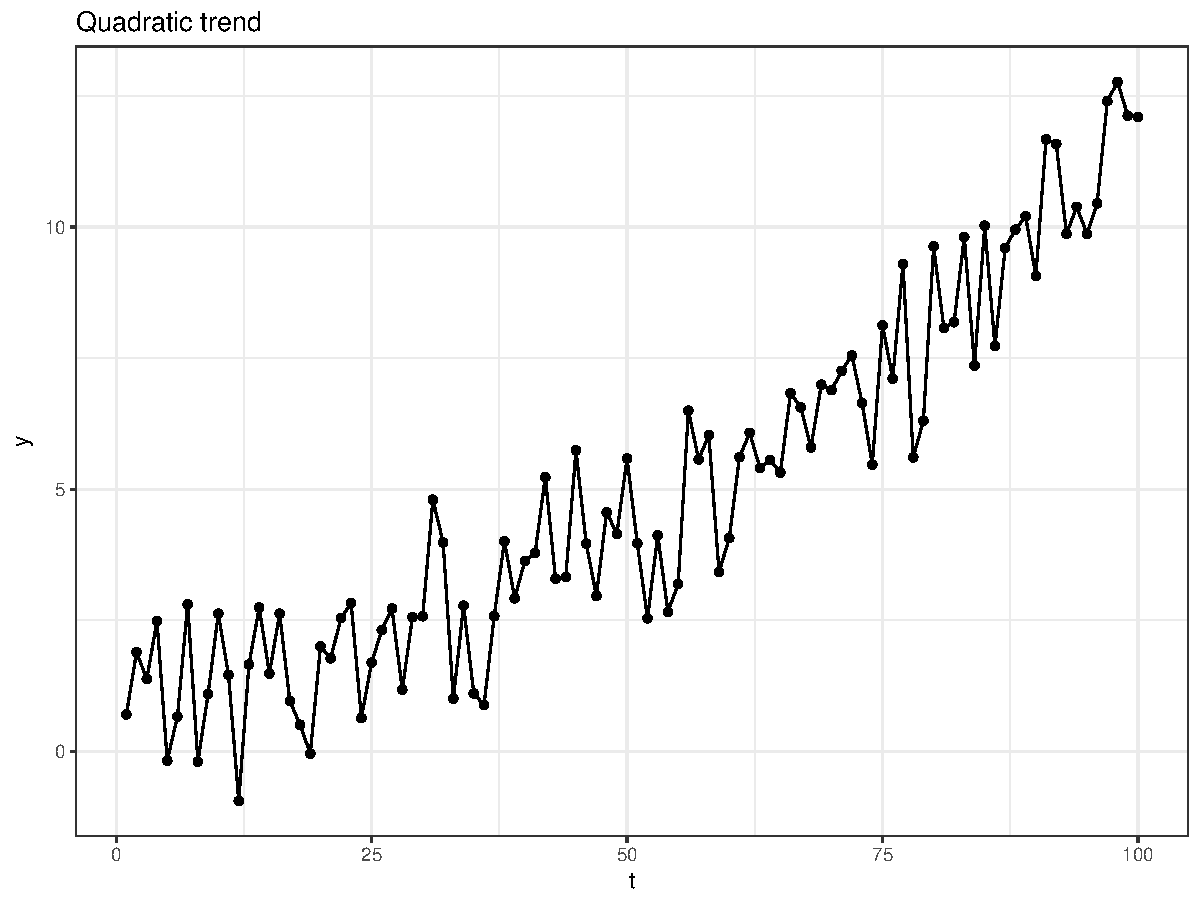
\includegraphics{Lec7_files/figure-beamer/unnamed-chunk-16-1.pdf}

\end{frame}

\begin{frame}{Detrending}

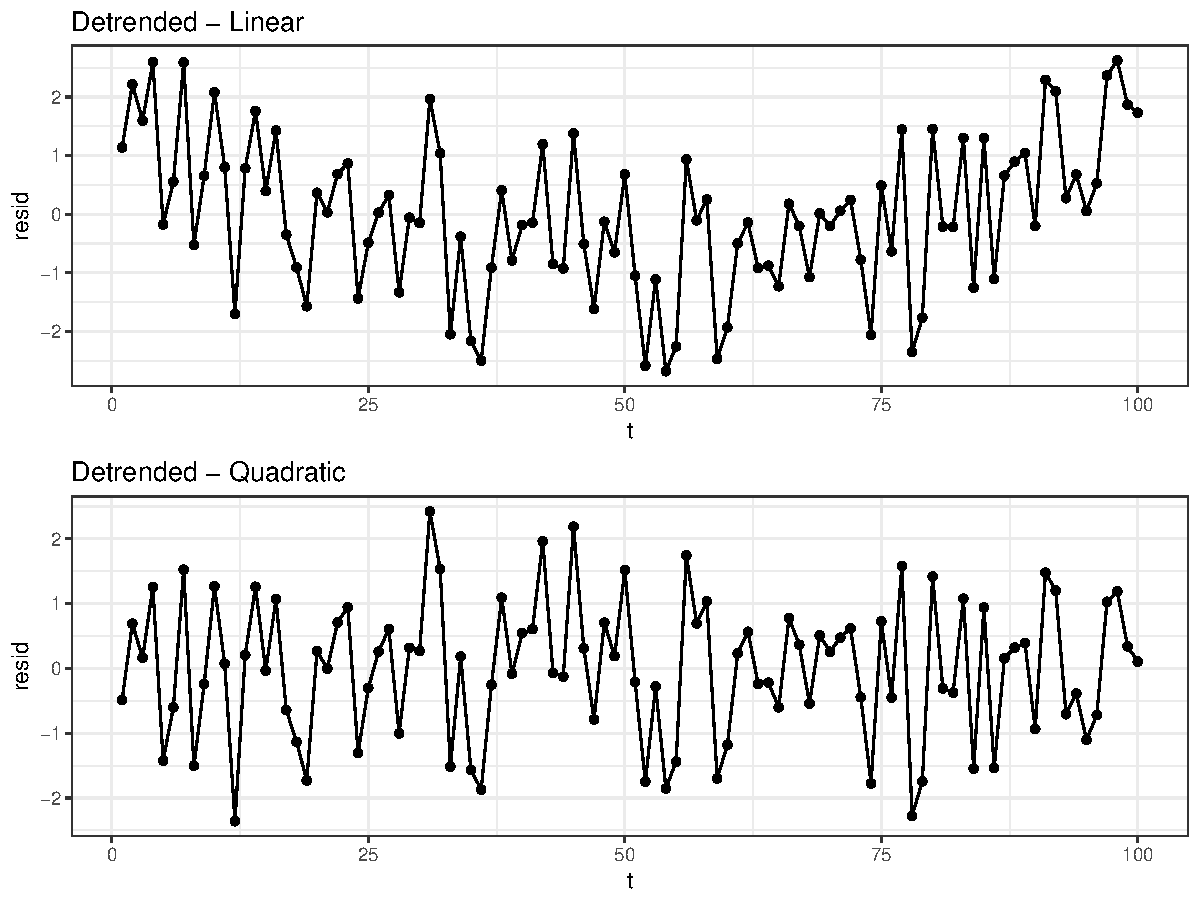
\includegraphics{Lec7_files/figure-beamer/unnamed-chunk-17-1.pdf}

\end{frame}

\begin{frame}[t]{2nd order differencing}

Let \(d_t = y_t - y_{t-1}\) be a first order difference then
\(d_t - d_{t-1}\) is a 2nd order difference.

\end{frame}

\begin{frame}{Differencing}

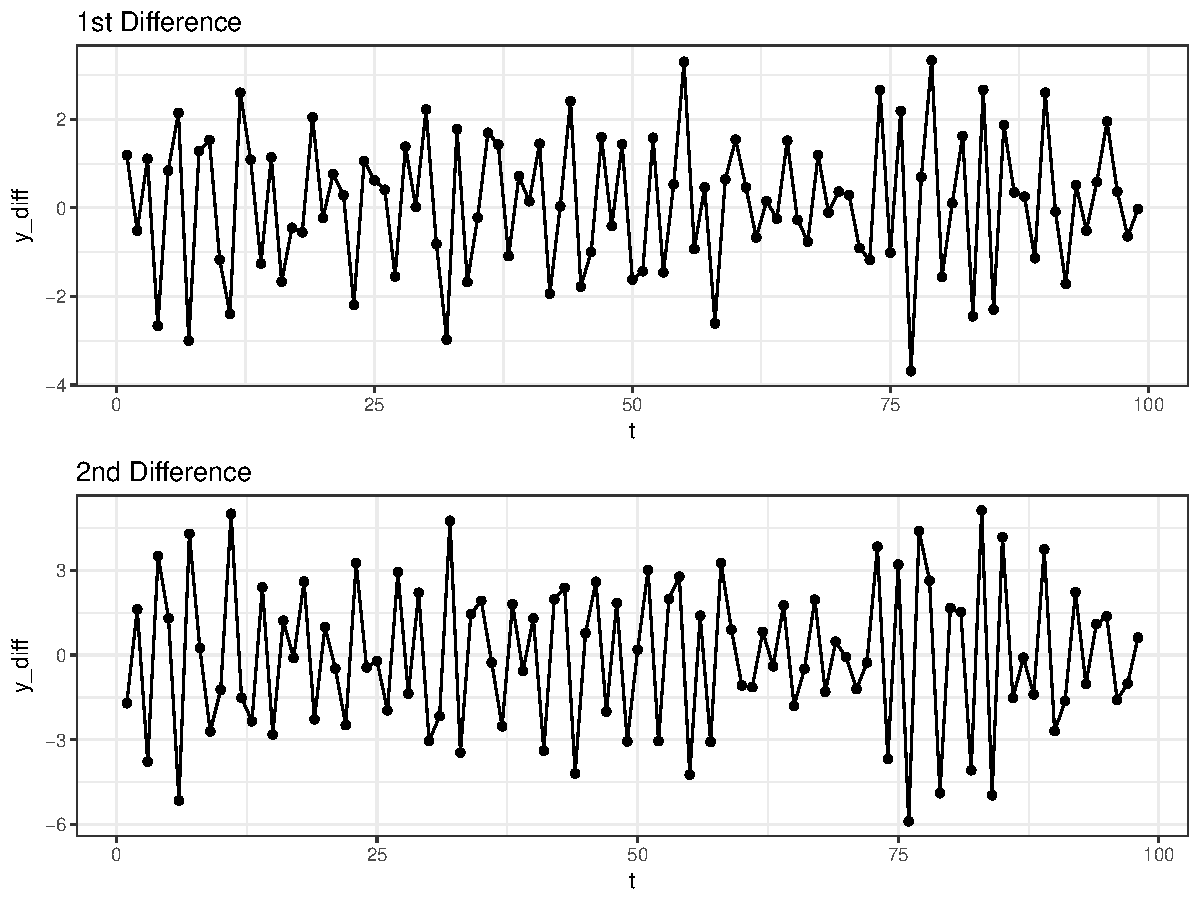
\includegraphics{Lec7_files/figure-beamer/unnamed-chunk-18-1.pdf}

\end{frame}

\begin{frame}{Differencing - ACF}

\begin{center}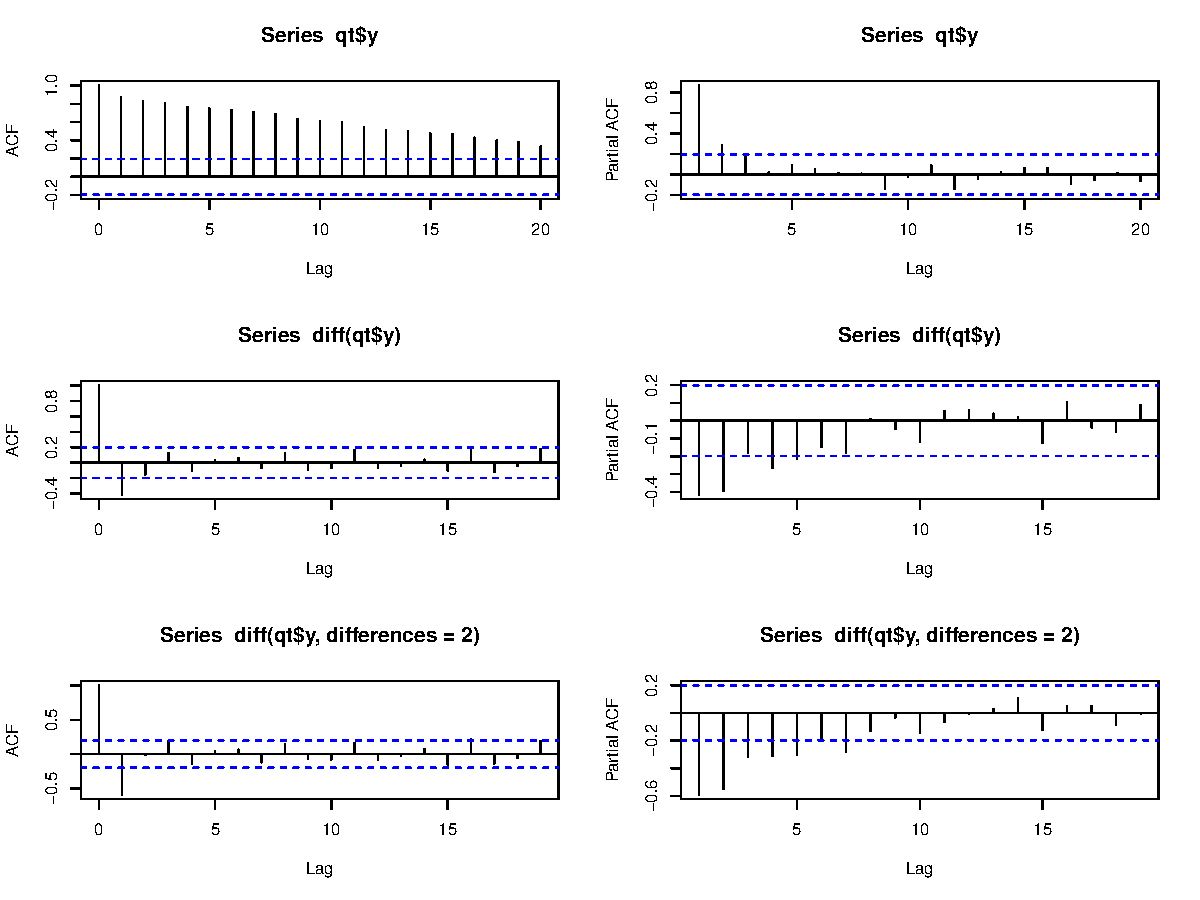
\includegraphics{Lec7_files/figure-beamer/unnamed-chunk-19-1} \end{center}

\end{frame}

\section{AR Models}\label{ar-models}

\begin{frame}{AR(1)}

Last time we mentioned a random walk with trend process where
\(y_t = \delta + y_{t-1} + w_t\). The AR(1) process is a slight
variation of this where we add a coefficient in front of the \(y_{t-1}\)
term. \[AR(1): \quad y_t = \delta + \phi \, y_{t-1} + w_t \]

\begin{center}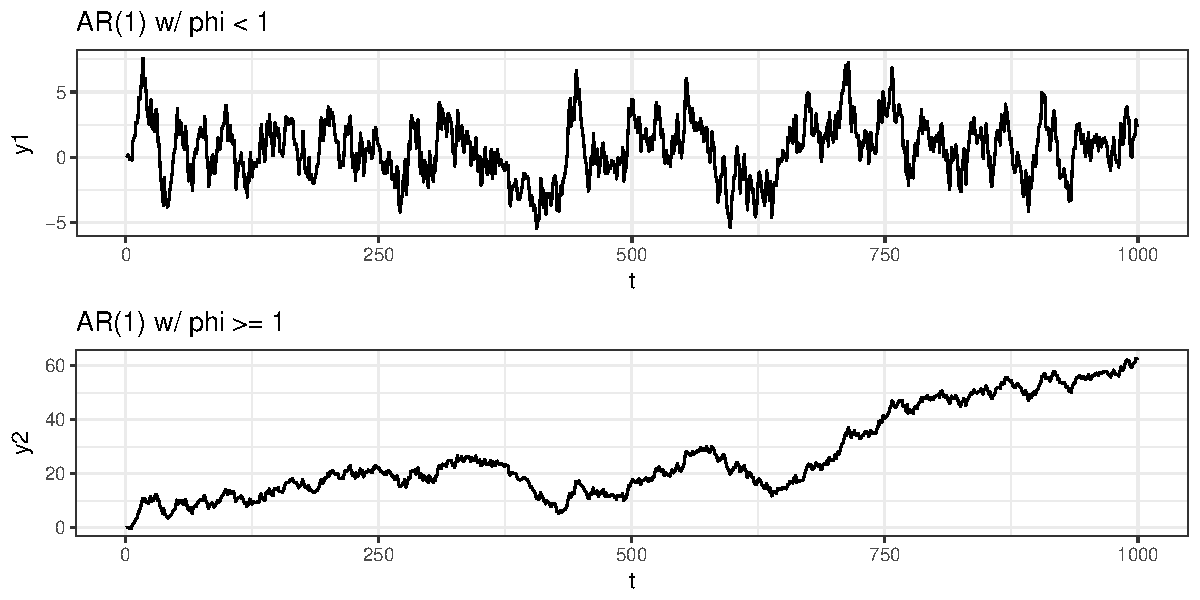
\includegraphics[width=0.8\textwidth]{Lec7_files/figure-beamer/unnamed-chunk-20-1} \end{center}

\end{frame}

\begin{frame}[t]{Stationarity}

Lets rewrite the AR(1) without any autoregressive terms

\end{frame}

\begin{frame}[t]{Differencing}

Once again we can examine differences of the response variable
\(y_t - y_{t-1}\) to attempt to achieve stationarity,s

\end{frame}

\begin{frame}{Identifying AR(1) Processes}

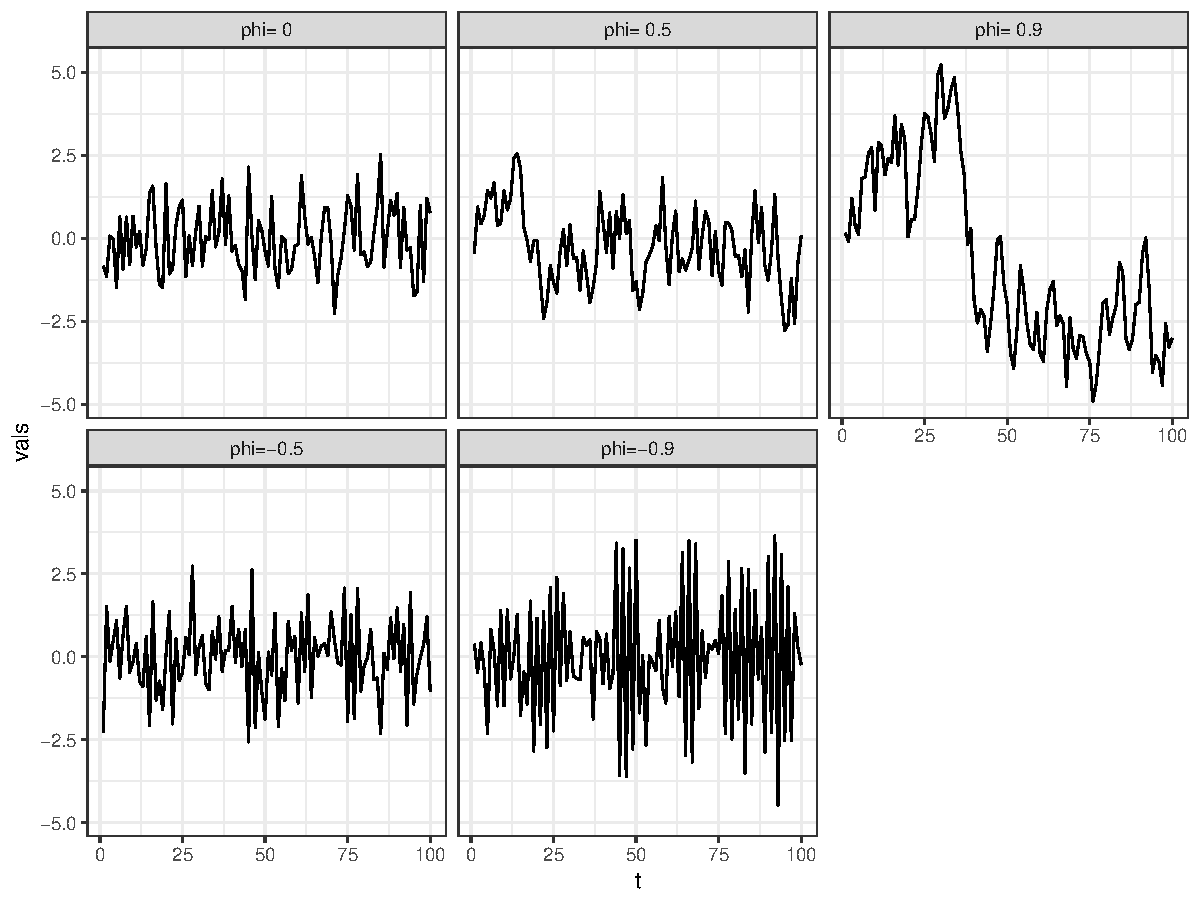
\includegraphics{Lec7_files/figure-beamer/unnamed-chunk-21-1.pdf}

\end{frame}

\begin{frame}{Identifying AR(1) Processes - ACFs}

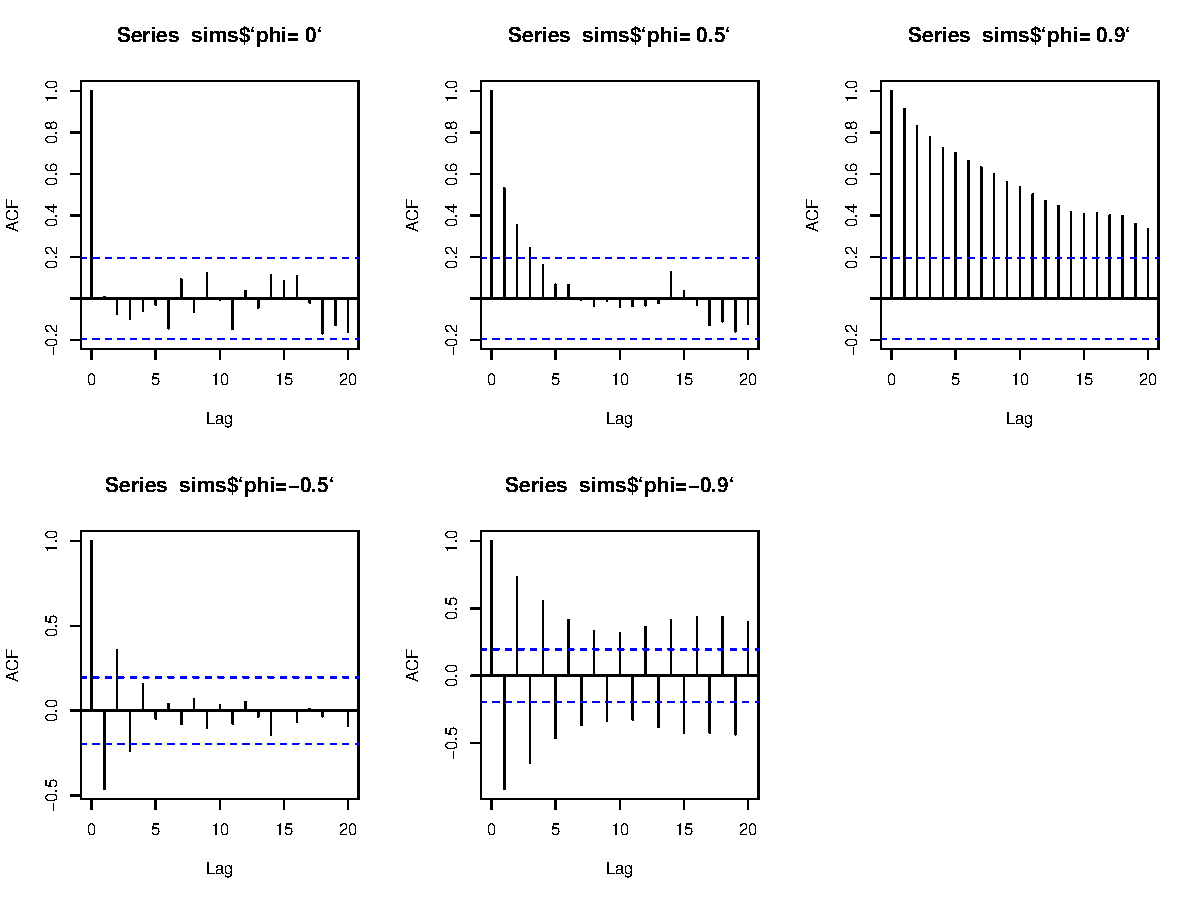
\includegraphics{Lec7_files/figure-beamer/unnamed-chunk-22-1.pdf}

\end{frame}

\begin{frame}[t]{AR(p) models}

We can easily generalize from an AR(1) to an AR(p) model by simply
adding additional autoregressive terms to the model.

\[ 
\begin{aligned}
AR(p): \quad y_t 
  &= \delta + \phi_1 \, y_{t-1} + \phi_2 \, y_{t-2} + \cdots + \phi_p \, y_{t-p} + w_t  \\
  &= \delta + w_t + \sum_{i=1}^p \phi_i \, y_{t-i}
\end{aligned}
\]

More on these next time.

\end{frame}

\end{document}
